% --- Program Section ---

\newprogram{Program 13}{Create a TSPSolver class with solve-tsp(dist-matrix: List[List[int]]) -> int taking an
adjacency matrix and returning the minimum tour cost.}

\subsection*{Code}


\begin{lstlisting}[language=python]
from typing import List


class TSPSolver:

    def solve_tsp(self, dist_matrix: List[List[int]]) -> int:
        n = len(dist_matrix)

        if n == 0:
            return 0

        # dp[mask][i] = minimum cost to visit all cities
        # in mask and end at city i
        dp = [[float('inf')] * n for _ in range(1 << n)]

        # Start from city 0
        dp[1][0] = 0

        for mask in range(1 << n):
            for current in range(n):

                if dp[mask][current] == float('inf'):
                    continue

                # Try visiting every unvisited city
                for next_city in range(n):

                    if mask & (1 << next_city):
                        continue

                    new_mask = mask | (1 << next_city)

                    new_cost = (
                        dp[mask][current]
                        + dist_matrix[current][next_city]
                    )

                    dp[new_mask][next_city] = min(
                        dp[new_mask][next_city],
                        new_cost
                    )

        # All cities visited
        full_mask = (1 << n) - 1

        # Return to starting city
        answer = float('inf')

        for city in range(1, n):
            answer = min(
                answer,
                dp[full_mask][city] + dist_matrix[city][0]
            )

        return answer


# -------------------------
# Example
# -------------------------

dist_matrix = [
    [0, 10, 15, 20],
    [10, 0, 35, 25],
    [15, 35, 0, 30],
    [20, 25, 30, 0]
]

solver = TSPSolver()

print("Minimum tour cost:",
      solver.solve_tsp(dist_matrix))
\end{lstlisting}

\subsection*{Output}
\begin{center}
    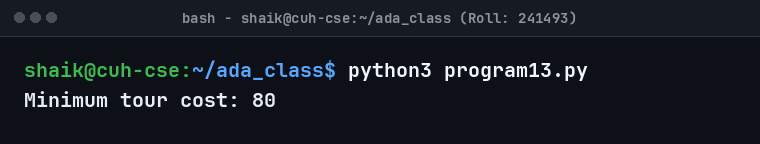
\includegraphics[width=0.88\textwidth]{Images/output_screenshot13.png}
\end{center}

\subsection*{GitHub Scan Code}
\begin{center}
    \begin{minipage}{0.3\textwidth}
        \centering
        % Generates a 2.5cm high QR code directly linking to the code file
        \qrcode[height=3.5cm]{https://github.com/gytdrop/ada_class/blob/main/program13.py} \\[0.2cm]
        \scriptsize\ttfamily Scan to view source code 
    \end{minipage}
\end{center}


% Add a horizontal line that indicates the END of the program.
\vspace{1cm}
\begin{center}
    \rule{1\textwidth}{1pt} % Clean, centered 1pt thick horizontal line
\end{center}